\documentclass[1p]{elsarticle_modified}
%\bibliographystyle{elsarticle-num}

%\usepackage[colorlinks]{hyperref}
%\usepackage{abbrmath_seonhwa} %\Abb, \Ascr, \Acal ,\Abf, \Afrak
\usepackage{amsfonts}
\usepackage{amssymb}
\usepackage{amsmath}
\usepackage{amsthm}
\usepackage{scalefnt}
\usepackage{amsbsy}
\usepackage{kotex}
\usepackage{caption}
\usepackage{subfig}
\usepackage{color}
\usepackage{graphicx}
\usepackage{xcolor} %% white, black, red, green, blue, cyan, magenta, yellow
\usepackage{float}
\usepackage{setspace}
\usepackage{hyperref}

\usepackage{tikz}
\usetikzlibrary{arrows}

\usepackage{multirow}
\usepackage{array} % fixed length table
\usepackage{hhline}

%%%%%%%%%%%%%%%%%%%%%
\makeatletter
\renewcommand*\env@matrix[1][\arraystretch]{%
	\edef\arraystretch{#1}%
	\hskip -\arraycolsep
	\let\@ifnextchar\new@ifnextchar
	\array{*\c@MaxMatrixCols c}}
\makeatother %https://tex.stackexchange.com/questions/14071/how-can-i-increase-the-line-spacing-in-a-matrix
%%%%%%%%%%%%%%%

\usepackage[normalem]{ulem}

\newcommand{\msout}[1]{\ifmmode\text{\sout{\ensuremath{#1}}}\else\sout{#1}\fi}
%SOURCE: \msout is \stkout macro in https://tex.stackexchange.com/questions/20609/strikeout-in-math-mode

\newcommand{\cancel}[1]{
	\ifmmode
	{\color{red}\msout{#1}}
	\else
	{\color{red}\sout{#1}}
	\fi
}

\newcommand{\add}[1]{
	{\color{blue}\uwave{#1}}
}

\newcommand{\replace}[2]{
	\ifmmode
	{\color{red}\msout{#1}}{\color{blue}\uwave{#2}}
	\else
	{\color{red}\sout{#1}}{\color{blue}\uwave{#2}}
	\fi
}

\newcommand{\Sol}{\mathcal{S}} %segment
\newcommand{\D}{D} %diagram
\newcommand{\A}{\mathcal{A}} %arc


%%%%%%%%%%%%%%%%%%%%%%%%%%%%%5 test

\def\sl{\operatorname{\textup{SL}}(2,\Cbb)}
\def\psl{\operatorname{\textup{PSL}}(2,\Cbb)}
\def\quan{\mkern 1mu \triangleright \mkern 1mu}

\theoremstyle{definition}
\newtheorem{thm}{Theorem}[section]
\newtheorem{prop}[thm]{Proposition}
\newtheorem{lem}[thm]{Lemma}
\newtheorem{ques}[thm]{Question}
\newtheorem{cor}[thm]{Corollary}
\newtheorem{defn}[thm]{Definition}
\newtheorem{exam}[thm]{Example}
\newtheorem{rmk}[thm]{Remark}
\newtheorem{alg}[thm]{Algorithm}

\newcommand{\I}{\sqrt{-1}}
\begin{document}

%\begin{frontmatter}
%
%\title{Boundary parabolic representations of knots up to 8 crossings}
%
%%% Group authors per affiliation:
%\author{Yunhi Cho} 
%\address{Department of Mathematics, University of Seoul, Seoul, Korea}
%\ead{yhcho@uos.ac.kr}
%
%
%\author{Seonhwa Kim} %\fnref{s_kim}}
%\address{Center for Geometry and Physics, Institute for Basic Science, Pohang, 37673, Korea}
%\ead{ryeona17@ibs.re.kr}
%
%\author{Hyuk Kim}
%\address{Department of Mathematical Sciences, Seoul National University, Seoul 08826, Korea}
%\ead{hyukkim@snu.ac.kr}
%
%\author{Seokbeom Yoon}
%\address{Department of Mathematical Sciences, Seoul National University, Seoul, 08826,  Korea}
%\ead{sbyoon15@snu.ac.kr}
%
%\begin{abstract}
%We find all boundary parabolic representation of knots up to 8 crossings.
%
%\end{abstract}
%\begin{keyword}
%    \MSC[2010] 57M25 
%\end{keyword}
%
%\end{frontmatter}

%\linenumbers
%\tableofcontents
%
\newcommand\colored[1]{\textcolor{white}{\rule[-0.35ex]{0.8em}{1.4ex}}\kern-0.8em\color{red} #1}%
%\newcommand\colored[1]{\textcolor{white}{ #1}\kern-2.17ex	\textcolor{white}{ #1}\kern-1.81ex	\textcolor{white}{ #1}\kern-2.15ex\color{red}#1	}

{\Large $\underline{12a_{0305}~(K12a_{0305})}$}

\setlength{\tabcolsep}{10pt}
\renewcommand{\arraystretch}{1.6}
\vspace{1cm}\begin{tabular}{m{100pt}>{\centering\arraybackslash}m{274pt}}
\multirow{5}{120pt}{
	\centering
	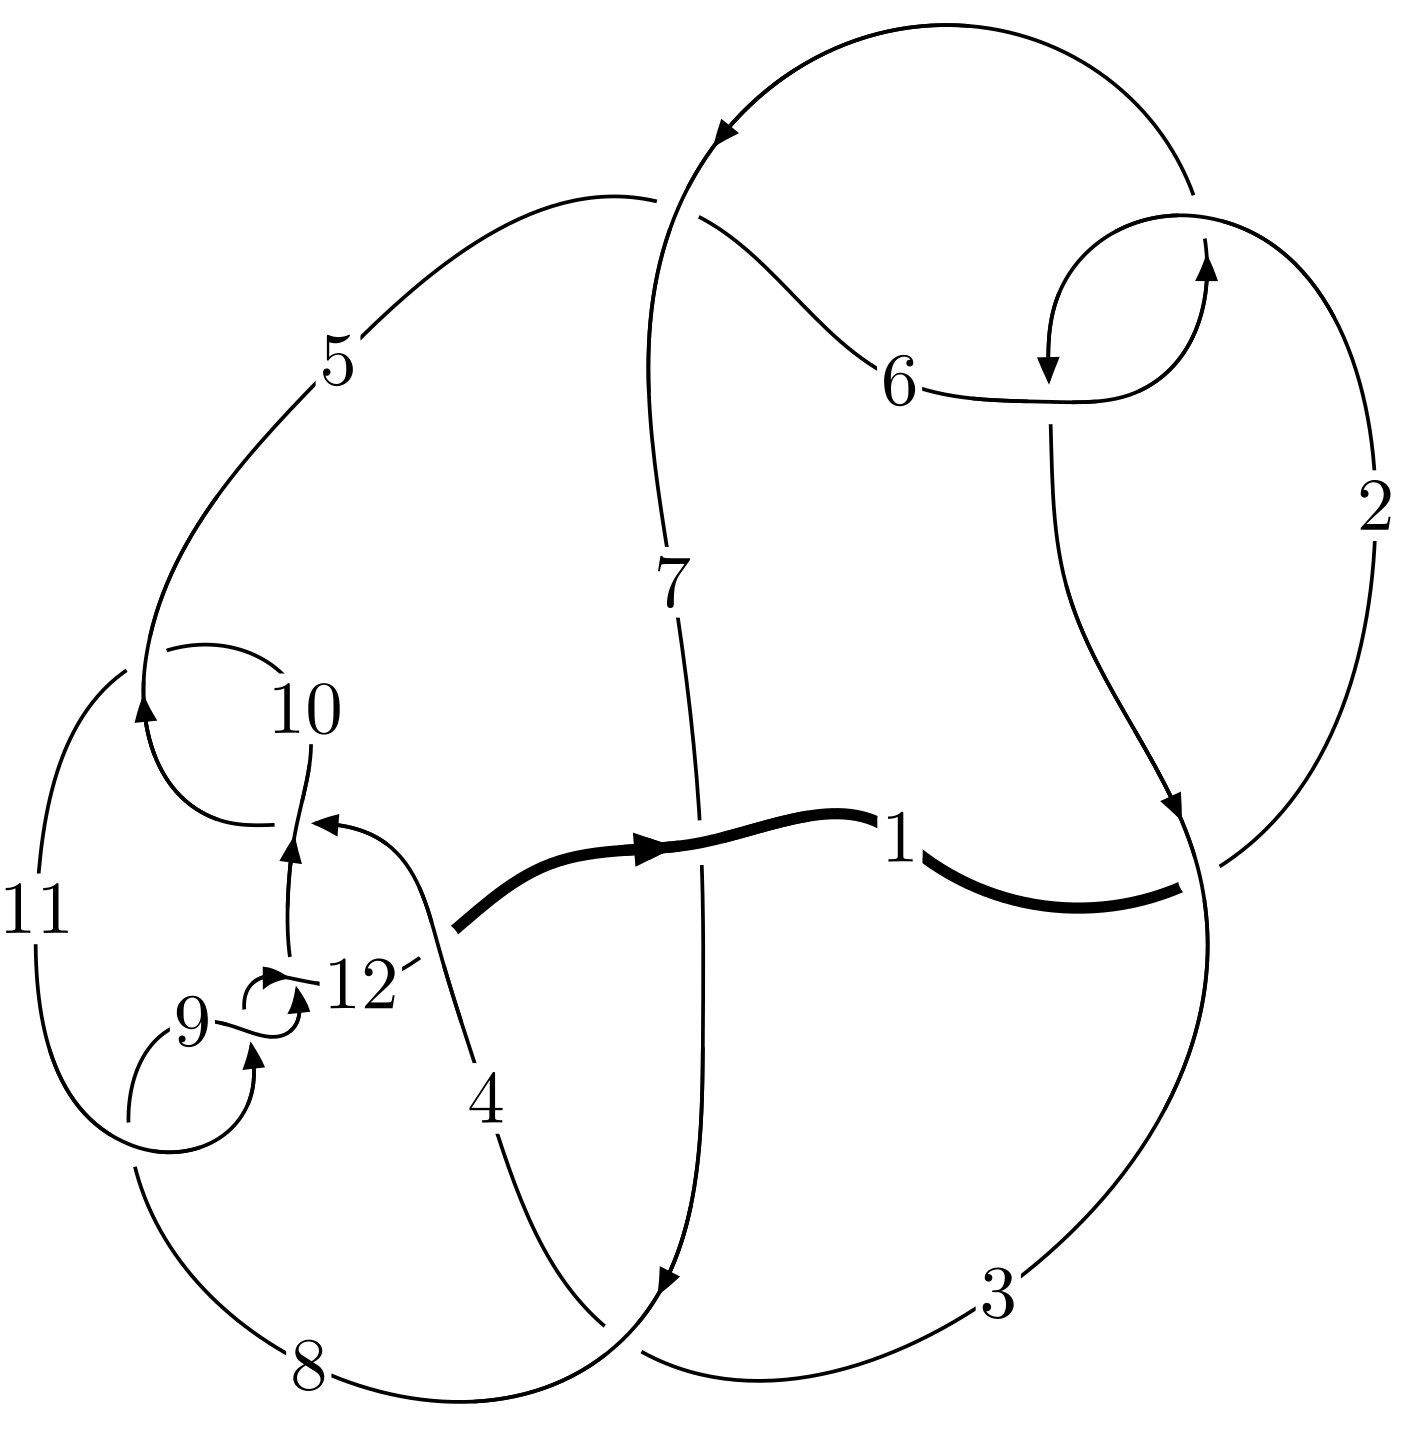
\includegraphics[width=112pt]{../../../GIT/diagram.site/Diagrams/png/1106_12a_0305.png}\\
\ \ \ A knot diagram\footnotemark}&
\allowdisplaybreaks
\textbf{Linearized knot diagam} \\
\cline{2-2}
 &
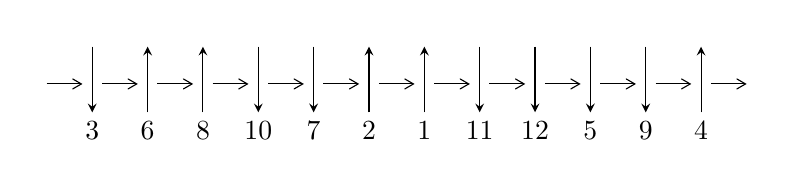
\begin{tikzpicture}[x=20pt, y=17pt]
	% nodes
	\node (C0) at (0, 0) {};
	\node (C1) at (1, 0) {};
	\node (C1U) at (1, +1) {};
	\node (C1D) at (1, -1) {3};

	\node (C2) at (2, 0) {};
	\node (C2U) at (2, +1) {};
	\node (C2D) at (2, -1) {6};

	\node (C3) at (3, 0) {};
	\node (C3U) at (3, +1) {};
	\node (C3D) at (3, -1) {8};

	\node (C4) at (4, 0) {};
	\node (C4U) at (4, +1) {};
	\node (C4D) at (4, -1) {10};

	\node (C5) at (5, 0) {};
	\node (C5U) at (5, +1) {};
	\node (C5D) at (5, -1) {7};

	\node (C6) at (6, 0) {};
	\node (C6U) at (6, +1) {};
	\node (C6D) at (6, -1) {2};

	\node (C7) at (7, 0) {};
	\node (C7U) at (7, +1) {};
	\node (C7D) at (7, -1) {1};

	\node (C8) at (8, 0) {};
	\node (C8U) at (8, +1) {};
	\node (C8D) at (8, -1) {11};

	\node (C9) at (9, 0) {};
	\node (C9U) at (9, +1) {};
	\node (C9D) at (9, -1) {12};

	\node (C10) at (10, 0) {};
	\node (C10U) at (10, +1) {};
	\node (C10D) at (10, -1) {5};

	\node (C11) at (11, 0) {};
	\node (C11U) at (11, +1) {};
	\node (C11D) at (11, -1) {9};

	\node (C12) at (12, 0) {};
	\node (C12U) at (12, +1) {};
	\node (C12D) at (12, -1) {4};
	\node (C13) at (13, 0) {};

	% arrows
	\draw[->,>={angle 60}]
	(C0) edge (C1) (C1) edge (C2) (C2) edge (C3) (C3) edge (C4) (C4) edge (C5) (C5) edge (C6) (C6) edge (C7) (C7) edge (C8) (C8) edge (C9) (C9) edge (C10) (C10) edge (C11) (C11) edge (C12) (C12) edge (C13) ;	\draw[->,>=stealth]
	(C1U) edge (C1D) (C2D) edge (C2U) (C3D) edge (C3U) (C4U) edge (C4D) (C5U) edge (C5D) (C6D) edge (C6U) (C7D) edge (C7U) (C8U) edge (C8D) (C9U) edge (C9D) (C10U) edge (C10D) (C11U) edge (C11D) (C12D) edge (C12U) ;
	\end{tikzpicture} \\
\hhline{~~} \\& 
\textbf{Solving Sequence} \\ \cline{2-2} 
 &
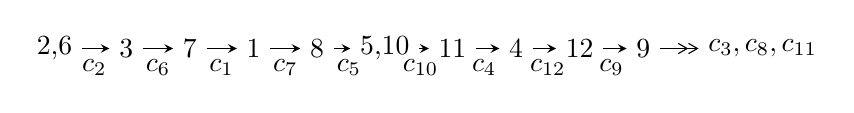
\begin{tikzpicture}[x=23pt, y=7pt]
	% node
	\node (A0) at (-1/8, 0) {2,6};
	\node (A1) at (1, 0) {3};
	\node (A2) at (2, 0) {7};
	\node (A3) at (3, 0) {1};
	\node (A4) at (4, 0) {8};
	\node (A5) at (81/16, 0) {5,10};
	\node (A6) at (49/8, 0) {11};
	\node (A7) at (57/8, 0) {4};
	\node (A8) at (65/8, 0) {12};
	\node (A9) at (73/8, 0) {9};
	\node (C1) at (1/2, -1) {$c_{2}$};
	\node (C2) at (3/2, -1) {$c_{6}$};
	\node (C3) at (5/2, -1) {$c_{1}$};
	\node (C4) at (7/2, -1) {$c_{7}$};
	\node (C5) at (9/2, -1) {$c_{5}$};
	\node (C6) at (45/8, -1) {$c_{10}$};
	\node (C7) at (53/8, -1) {$c_{4}$};
	\node (C8) at (61/8, -1) {$c_{12}$};
	\node (C9) at (69/8, -1) {$c_{9}$};
	\node (A10) at (11, 0) {$c_{3},c_{8},c_{11}$};

	% edge
	\draw[->,>=stealth]	
	(A0) edge (A1) (A1) edge (A2) (A2) edge (A3) (A3) edge (A4) (A4) edge (A5) (A5) edge (A6) (A6) edge (A7) (A7) edge (A8) (A8) edge (A9) ;
	\draw[->>,>={angle 60}]	
	(A9) edge (A10);
\end{tikzpicture} \\ 

\end{tabular} \\

\footnotetext{
The image of knot diagram is generated by the software ``\textbf{Draw programme}" developed by Andrew Bartholomew(\url{http://www.layer8.co.uk/maths/draw/index.htm\#Running-draw}), where we modified some parts for our purpose(\url{https://github.com/CATsTAILs/LinksPainter}).
}\phantom \\ \newline 
\centering \textbf{Ideals for irreducible components\footnotemark of $X_{\text{par}}$} 
 
\begin{align*}
I^u_{1}&=\langle 
- u^{89}- u^{88}+\cdots+b-2 u,\;u^{87}+14 u^{85}+\cdots+a+1,\;u^{92}+2 u^{91}+\cdots+3 u-1\rangle \\
I^u_{2}&=\langle 
u^8- u^7+u^6- u^5+u^4- u^3+b- u,\;- u^6- u^4- u^2+a- u,\;u^9- u^8+2 u^7- u^6+3 u^5- u^4+2 u^3+u+1\rangle \\
\\
\end{align*}
\raggedright * 2 irreducible components of $\dim_{\mathbb{C}}=0$, with total 101 representations.\\
\footnotetext{All coefficients of polynomials are rational numbers. But the coefficients are sometimes approximated in decimal forms when there is not enough margin.}
\newpage
\renewcommand{\arraystretch}{1}
\centering \section*{I. $I^u_{1}= \langle - u^{89}- u^{88}+\cdots+b-2 u,\;u^{87}+14 u^{85}+\cdots+a+1,\;u^{92}+2 u^{91}+\cdots+3 u-1 \rangle$}
\flushleft \textbf{(i) Arc colorings}\\
\begin{tabular}{m{7pt} m{180pt} m{7pt} m{180pt} }
\flushright $a_{2}=$&$\begin{pmatrix}1\\0\end{pmatrix}$ \\
\flushright $a_{6}=$&$\begin{pmatrix}0\\u\end{pmatrix}$ \\
\flushright $a_{3}=$&$\begin{pmatrix}1\\- u^2\end{pmatrix}$ \\
\flushright $a_{7}=$&$\begin{pmatrix}u\\u\end{pmatrix}$ \\
\flushright $a_{1}=$&$\begin{pmatrix}u^2+1\\- u^4\end{pmatrix}$ \\
\flushright $a_{8}=$&$\begin{pmatrix}u^7+2 u^5+2 u^3+2 u\\- u^9- u^7- u^5+u\end{pmatrix}$ \\
\flushright $a_{5}=$&$\begin{pmatrix}u^3\\u^3+u\end{pmatrix}$ \\
\flushright $a_{10}=$&$\begin{pmatrix}- u^{87}-14 u^{85}+\cdots-3 u-1\\u^{89}+u^{88}+\cdots+3 u^2+2 u\end{pmatrix}$ \\
\flushright $a_{11}=$&$\begin{pmatrix}2 u^{91}+2 u^{90}+\cdots+4 u^2-2\\2 u^{91}+u^{90}+\cdots+6 u^2+u\end{pmatrix}$ \\
\flushright $a_{4}=$&$\begin{pmatrix}- u^{14}-3 u^{12}-6 u^{10}-9 u^8-8 u^6-6 u^4-2 u^2+1\\u^{16}+2 u^{14}+4 u^{12}+4 u^{10}+2 u^8-2 u^4-2 u^2\end{pmatrix}$ \\
\flushright $a_{12}=$&$\begin{pmatrix}u^{26}+5 u^{24}+\cdots- u^2+1\\- u^{28}-4 u^{26}+\cdots+10 u^6+3 u^4\end{pmatrix}$ \\
\flushright $a_{9}=$&$\begin{pmatrix}u^{91}+u^{90}+\cdots+u^2-1\\u^{91}+u^{90}+\cdots+4 u^2+2 u\end{pmatrix}$\\&\end{tabular}
\flushleft \textbf{(ii) Obstruction class $= -1$}\\~\\
\flushleft \textbf{(iii) Cusp Shapes $= -4 u^{91}-2 u^{90}+\cdots+4 u-10$}\\~\\
\newpage\renewcommand{\arraystretch}{1}
\flushleft \textbf{(iv) u-Polynomials at the component}\newline \\
\begin{tabular}{m{50pt}|m{274pt}}
Crossings & \hspace{64pt}u-Polynomials at each crossing \\
\hline $$\begin{aligned}c_{1},c_{5}\end{aligned}$$&$\begin{aligned}
&u^{92}+30 u^{91}+\cdots-15 u+1
\end{aligned}$\\
\hline $$\begin{aligned}c_{2},c_{6}\end{aligned}$$&$\begin{aligned}
&u^{92}-2 u^{91}+\cdots-3 u-1
\end{aligned}$\\
\hline $$\begin{aligned}c_{3}\end{aligned}$$&$\begin{aligned}
&u^{92}-2 u^{91}+\cdots-19073 u-4777
\end{aligned}$\\
\hline $$\begin{aligned}c_{4},c_{10}\end{aligned}$$&$\begin{aligned}
&u^{92}- u^{91}+\cdots+512 u+512
\end{aligned}$\\
\hline $$\begin{aligned}c_{7}\end{aligned}$$&$\begin{aligned}
&u^{92}+10 u^{91}+\cdots-2595 u-175
\end{aligned}$\\
\hline $$\begin{aligned}c_{8},c_{9},c_{11}\end{aligned}$$&$\begin{aligned}
&u^{92}-10 u^{91}+\cdots+9 u-1
\end{aligned}$\\
\hline $$\begin{aligned}c_{12}\end{aligned}$$&$\begin{aligned}
&u^{92}+6 u^{91}+\cdots+93765 u+53361
\end{aligned}$\\
\hline
\end{tabular}\\~\\
\newpage\renewcommand{\arraystretch}{1}
\flushleft \textbf{(v) Riley Polynomials at the component}\newline \\
\begin{tabular}{m{50pt}|m{274pt}}
Crossings & \hspace{64pt}Riley Polynomials at each crossing \\
\hline $$\begin{aligned}c_{1},c_{5}\end{aligned}$$&$\begin{aligned}
&y^{92}+66 y^{91}+\cdots-223 y+1
\end{aligned}$\\
\hline $$\begin{aligned}c_{2},c_{6}\end{aligned}$$&$\begin{aligned}
&y^{92}+30 y^{91}+\cdots-15 y+1
\end{aligned}$\\
\hline $$\begin{aligned}c_{3}\end{aligned}$$&$\begin{aligned}
&y^{92}-18 y^{91}+\cdots-956098667 y+22819729
\end{aligned}$\\
\hline $$\begin{aligned}c_{4},c_{10}\end{aligned}$$&$\begin{aligned}
&y^{92}-57 y^{91}+\cdots-1835008 y+262144
\end{aligned}$\\
\hline $$\begin{aligned}c_{7}\end{aligned}$$&$\begin{aligned}
&y^{92}+6 y^{91}+\cdots+948825 y+30625
\end{aligned}$\\
\hline $$\begin{aligned}c_{8},c_{9},c_{11}\end{aligned}$$&$\begin{aligned}
&y^{92}-90 y^{91}+\cdots-3 y+1
\end{aligned}$\\
\hline $$\begin{aligned}c_{12}\end{aligned}$$&$\begin{aligned}
&y^{92}+42 y^{91}+\cdots-115995084723 y+2847396321
\end{aligned}$\\
\hline
\end{tabular}\\~\\
\newpage\flushleft \textbf{(vi) Complex Volumes and Cusp Shapes}
$$\begin{array}{c|c|c}  
\text{Solutions to }I^u_{1}& \I (\text{vol} + \sqrt{-1}CS) & \text{Cusp shape}\\
 \hline 
\begin{aligned}
u &= -0.238579 + 0.976043 I \\
a &= \phantom{-}0.192909 - 0.693401 I \\
b &= -0.304491 - 0.860553 I\end{aligned}
 & -5.41288 - 2.84467 I & \phantom{-0.000000 } 0 \\ \hline\begin{aligned}
u &= -0.238579 - 0.976043 I \\
a &= \phantom{-}0.192909 + 0.693401 I \\
b &= -0.304491 + 0.860553 I\end{aligned}
 & -5.41288 + 2.84467 I & \phantom{-0.000000 } 0 \\ \hline\begin{aligned}
u &= -0.131476 + 0.996623 I \\
a &= \phantom{-}0.210814 + 0.343582 I \\
b &= \phantom{-}0.521220 + 0.022009 I\end{aligned}
 & -2.04930 - 2.60188 I & \phantom{-0.000000 } 0 \\ \hline\begin{aligned}
u &= -0.131476 - 0.996623 I \\
a &= \phantom{-}0.210814 - 0.343582 I \\
b &= \phantom{-}0.521220 - 0.022009 I\end{aligned}
 & -2.04930 + 2.60188 I & \phantom{-0.000000 } 0 \\ \hline\begin{aligned}
u &= -0.761512 + 0.636187 I \\
a &= \phantom{-}0.16026 - 2.38247 I \\
b &= \phantom{-}1.56743 - 1.52368 I\end{aligned}
 & -7.42452 - 1.21614 I & \phantom{-0.000000 } 0 \\ \hline\begin{aligned}
u &= -0.761512 - 0.636187 I \\
a &= \phantom{-}0.16026 + 2.38247 I \\
b &= \phantom{-}1.56743 + 1.52368 I\end{aligned}
 & -7.42452 + 1.21614 I & \phantom{-0.000000 } 0 \\ \hline\begin{aligned}
u &= -0.781538 + 0.684375 I \\
a &= \phantom{-}0.25605 + 2.82276 I \\
b &= -1.81816 + 2.53546 I\end{aligned}
 & \phantom{-}0.155477 + 1.294890 I & \phantom{-0.000000 } 0 \\ \hline\begin{aligned}
u &= -0.781538 - 0.684375 I \\
a &= \phantom{-}0.25605 - 2.82276 I \\
b &= -1.81816 - 2.53546 I\end{aligned}
 & \phantom{-}0.155477 - 1.294890 I & \phantom{-0.000000 } 0 \\ \hline\begin{aligned}
u &= \phantom{-}0.098394 + 1.038460 I \\
a &= \phantom{-}0.07502 + 1.54246 I \\
b &= \phantom{-}0.567259 - 0.826734 I\end{aligned}
 & -5.85938 + 1.27529 I & \phantom{-0.000000 } 0 \\ \hline\begin{aligned}
u &= \phantom{-}0.098394 - 1.038460 I \\
a &= \phantom{-}0.07502 - 1.54246 I \\
b &= \phantom{-}0.567259 + 0.826734 I\end{aligned}
 & -5.85938 - 1.27529 I & \phantom{-0.000000 } 0\\
 \hline 
 \end{array}$$\newpage$$\begin{array}{c|c|c}  
\text{Solutions to }I^u_{1}& \I (\text{vol} + \sqrt{-1}CS) & \text{Cusp shape}\\
 \hline 
\begin{aligned}
u &= \phantom{-}0.796526 + 0.681227 I \\
a &= \phantom{-}1.180110 - 0.586282 I \\
b &= -0.184618 - 1.380540 I\end{aligned}
 & -1.36598 - 3.95919 I & \phantom{-0.000000 } 0 \\ \hline\begin{aligned}
u &= \phantom{-}0.796526 - 0.681227 I \\
a &= \phantom{-}1.180110 + 0.586282 I \\
b &= -0.184618 + 1.380540 I\end{aligned}
 & -1.36598 + 3.95919 I & \phantom{-0.000000 } 0 \\ \hline\begin{aligned}
u &= -0.113967 + 1.047090 I \\
a &= -0.317702 - 0.526590 I \\
b &= -0.972673 + 0.055257 I\end{aligned}
 & -7.57114 - 3.91705 I & \phantom{-0.000000 } 0 \\ \hline\begin{aligned}
u &= -0.113967 - 1.047090 I \\
a &= -0.317702 + 0.526590 I \\
b &= -0.972673 - 0.055257 I\end{aligned}
 & -7.57114 + 3.91705 I & \phantom{-0.000000 } 0 \\ \hline\begin{aligned}
u &= \phantom{-}0.128444 + 1.048180 I \\
a &= \phantom{-}0.42689 - 1.60839 I \\
b &= -0.356284 + 0.752529 I\end{aligned}
 & -5.07389 + 6.38810 I & \phantom{-0.000000 } 0 \\ \hline\begin{aligned}
u &= \phantom{-}0.128444 - 1.048180 I \\
a &= \phantom{-}0.42689 + 1.60839 I \\
b &= -0.356284 - 0.752529 I\end{aligned}
 & -5.07389 - 6.38810 I & \phantom{-0.000000 } 0 \\ \hline\begin{aligned}
u &= -0.806783 + 0.685584 I \\
a &= \phantom{-}0.09380 - 3.06953 I \\
b &= \phantom{-}2.61016 - 2.39283 I\end{aligned}
 & \phantom{-}1.26879 + 6.37618 I & \phantom{-0.000000 } 0 \\ \hline\begin{aligned}
u &= -0.806783 - 0.685584 I \\
a &= \phantom{-}0.09380 + 3.06953 I \\
b &= \phantom{-}2.61016 + 2.39283 I\end{aligned}
 & \phantom{-}1.26879 - 6.37618 I & \phantom{-0.000000 } 0 \\ \hline\begin{aligned}
u &= -0.743166 + 0.754535 I \\
a &= \phantom{-}1.13339 + 1.20352 I \\
b &= \phantom{-}0.73726 + 1.94182 I\end{aligned}
 & \phantom{-}1.43085 + 0.04969 I & \phantom{-0.000000 } 0 \\ \hline\begin{aligned}
u &= -0.743166 - 0.754535 I \\
a &= \phantom{-}1.13339 - 1.20352 I \\
b &= \phantom{-}0.73726 - 1.94182 I\end{aligned}
 & \phantom{-}1.43085 - 0.04969 I & \phantom{-0.000000 } 0\\
 \hline 
 \end{array}$$\newpage$$\begin{array}{c|c|c}  
\text{Solutions to }I^u_{1}& \I (\text{vol} + \sqrt{-1}CS) & \text{Cusp shape}\\
 \hline 
\begin{aligned}
u &= -0.822268 + 0.680379 I \\
a &= -0.26921 + 3.00155 I \\
b &= -2.83495 + 2.02876 I\end{aligned}
 & -4.87607 + 10.56990 I & \phantom{-0.000000 } 0 \\ \hline\begin{aligned}
u &= -0.822268 - 0.680379 I \\
a &= -0.26921 - 3.00155 I \\
b &= -2.83495 - 2.02876 I\end{aligned}
 & -4.87607 - 10.56990 I & \phantom{-0.000000 } 0 \\ \hline\begin{aligned}
u &= \phantom{-}0.068444 + 1.066700 I \\
a &= -0.119803 - 1.063560 I \\
b &= -0.669699 + 0.996000 I\end{aligned}
 & -13.26790 - 1.71324 I & \phantom{-0.000000 } 0 \\ \hline\begin{aligned}
u &= \phantom{-}0.068444 - 1.066700 I \\
a &= -0.119803 + 1.063560 I \\
b &= -0.669699 - 0.996000 I\end{aligned}
 & -13.26790 + 1.71324 I & \phantom{-0.000000 } 0 \\ \hline\begin{aligned}
u &= \phantom{-}0.794586 + 0.715154 I \\
a &= -0.701553 + 0.368801 I \\
b &= \phantom{-}0.106681 + 0.861927 I\end{aligned}
 & \phantom{-}4.11451 - 2.13885 I & \phantom{-0.000000 } 0 \\ \hline\begin{aligned}
u &= \phantom{-}0.794586 - 0.715154 I \\
a &= -0.701553 - 0.368801 I \\
b &= \phantom{-}0.106681 - 0.861927 I\end{aligned}
 & \phantom{-}4.11451 + 2.13885 I & \phantom{-0.000000 } 0 \\ \hline\begin{aligned}
u &= \phantom{-}0.523406 + 0.932221 I \\
a &= -2.86628 + 1.08586 I \\
b &= -1.70161 + 2.54061 I\end{aligned}
 & -2.88968 - 0.50850 I & \phantom{-0.000000 } 0 \\ \hline\begin{aligned}
u &= \phantom{-}0.523406 - 0.932221 I \\
a &= -2.86628 - 1.08586 I \\
b &= -1.70161 - 2.54061 I\end{aligned}
 & -2.88968 + 0.50850 I & \phantom{-0.000000 } 0 \\ \hline\begin{aligned}
u &= -0.603531 + 0.883423 I \\
a &= -0.405753 + 0.377637 I \\
b &= -0.456391 + 0.312778 I\end{aligned}
 & \phantom{-}0.27502 - 2.36293 I & \phantom{-0.000000 } 0 \\ \hline\begin{aligned}
u &= -0.603531 - 0.883423 I \\
a &= -0.405753 - 0.377637 I \\
b &= -0.456391 - 0.312778 I\end{aligned}
 & \phantom{-}0.27502 + 2.36293 I & \phantom{-0.000000 } 0\\
 \hline 
 \end{array}$$\newpage$$\begin{array}{c|c|c}  
\text{Solutions to }I^u_{1}& \I (\text{vol} + \sqrt{-1}CS) & \text{Cusp shape}\\
 \hline 
\begin{aligned}
u &= \phantom{-}0.141577 + 1.066640 I \\
a &= -0.64547 + 1.36105 I \\
b &= \phantom{-}0.165043 - 0.846640 I\end{aligned}
 & -11.4205 + 10.4846 I & \phantom{-0.000000 } 0 \\ \hline\begin{aligned}
u &= \phantom{-}0.141577 - 1.066640 I \\
a &= -0.64547 - 1.36105 I \\
b &= \phantom{-}0.165043 + 0.846640 I\end{aligned}
 & -11.4205 - 10.4846 I & \phantom{-0.000000 } 0 \\ \hline\begin{aligned}
u &= \phantom{-}0.483733 + 0.961923 I \\
a &= \phantom{-}2.62934 - 0.98848 I \\
b &= \phantom{-}1.77034 - 2.05250 I\end{aligned}
 & -9.44292 - 4.26740 I & \phantom{-0.000000 } 0 \\ \hline\begin{aligned}
u &= \phantom{-}0.483733 - 0.961923 I \\
a &= \phantom{-}2.62934 + 0.98848 I \\
b &= \phantom{-}1.77034 + 2.05250 I\end{aligned}
 & -9.44292 + 4.26740 I & \phantom{-0.000000 } 0 \\ \hline\begin{aligned}
u &= \phantom{-}0.041839 + 0.919641 I \\
a &= \phantom{-}1.46421 + 0.47733 I \\
b &= \phantom{-}0.510800 - 0.847804 I\end{aligned}
 & -3.71389 + 0.94541 I & -10.08955 + 0. I\phantom{ +0.000000I} \\ \hline\begin{aligned}
u &= \phantom{-}0.041839 - 0.919641 I \\
a &= \phantom{-}1.46421 - 0.47733 I \\
b &= \phantom{-}0.510800 + 0.847804 I\end{aligned}
 & -3.71389 - 0.94541 I & -10.08955 + 0. I\phantom{ +0.000000I} \\ \hline\begin{aligned}
u &= \phantom{-}0.738617 + 0.792436 I \\
a &= \phantom{-}0.08397 + 1.76696 I \\
b &= \phantom{-}1.79864 + 0.87393 I\end{aligned}
 & \phantom{-}0.61740 + 2.17666 I & \phantom{-0.000000 } 0 \\ \hline\begin{aligned}
u &= \phantom{-}0.738617 - 0.792436 I \\
a &= \phantom{-}0.08397 - 1.76696 I \\
b &= \phantom{-}1.79864 - 0.87393 I\end{aligned}
 & \phantom{-}0.61740 - 2.17666 I & \phantom{-0.000000 } 0 \\ \hline\begin{aligned}
u &= \phantom{-}0.780023 + 0.757512 I \\
a &= -0.138766 - 1.011260 I \\
b &= -1.111500 - 0.321008 I\end{aligned}
 & \phantom{-}4.83837 - 0.28034 I & \phantom{-0.000000 } 0 \\ \hline\begin{aligned}
u &= \phantom{-}0.780023 - 0.757512 I \\
a &= -0.138766 + 1.011260 I \\
b &= -1.111500 + 0.321008 I\end{aligned}
 & \phantom{-}4.83837 + 0.28034 I & \phantom{-0.000000 } 0\\
 \hline 
 \end{array}$$\newpage$$\begin{array}{c|c|c}  
\text{Solutions to }I^u_{1}& \I (\text{vol} + \sqrt{-1}CS) & \text{Cusp shape}\\
 \hline 
\begin{aligned}
u &= -0.545981 + 0.946335 I \\
a &= \phantom{-}0.786190 - 0.801145 I \\
b &= \phantom{-}0.983452 - 0.814754 I\end{aligned}
 & -5.14496 - 1.95841 I & \phantom{-0.000000 } 0 \\ \hline\begin{aligned}
u &= -0.545981 - 0.946335 I \\
a &= \phantom{-}0.786190 + 0.801145 I \\
b &= \phantom{-}0.983452 + 0.814754 I\end{aligned}
 & -5.14496 + 1.95841 I & \phantom{-0.000000 } 0 \\ \hline\begin{aligned}
u &= \phantom{-}0.819340 + 0.747466 I \\
a &= \phantom{-}0.811111 + 0.583349 I \\
b &= \phantom{-}0.969514 - 0.641469 I\end{aligned}
 & \phantom{-}1.33460 - 1.79462 I & \phantom{-0.000000 } 0 \\ \hline\begin{aligned}
u &= \phantom{-}0.819340 - 0.747466 I \\
a &= \phantom{-}0.811111 - 0.583349 I \\
b &= \phantom{-}0.969514 + 0.641469 I\end{aligned}
 & \phantom{-}1.33460 + 1.79462 I & \phantom{-0.000000 } 0 \\ \hline\begin{aligned}
u &= \phantom{-}0.569272 + 0.952059 I \\
a &= \phantom{-}3.05755 - 0.71634 I \\
b &= \phantom{-}2.21583 - 2.69381 I\end{aligned}
 & -3.18636 + 4.50271 I & \phantom{-0.000000 } 0 \\ \hline\begin{aligned}
u &= \phantom{-}0.569272 - 0.952059 I \\
a &= \phantom{-}3.05755 + 0.71634 I \\
b &= \phantom{-}2.21583 + 2.69381 I\end{aligned}
 & -3.18636 - 4.50271 I & \phantom{-0.000000 } 0 \\ \hline\begin{aligned}
u &= -0.765440 + 0.803103 I \\
a &= -0.818029 - 0.295898 I \\
b &= -1.30883 - 0.73438 I\end{aligned}
 & \phantom{-}3.29801 - 4.00356 I & \phantom{-0.000000 } 0 \\ \hline\begin{aligned}
u &= -0.765440 - 0.803103 I \\
a &= -0.818029 + 0.295898 I \\
b &= -1.30883 + 0.73438 I\end{aligned}
 & \phantom{-}3.29801 + 4.00356 I & \phantom{-0.000000 } 0 \\ \hline\begin{aligned}
u &= -0.133642 + 0.866499 I \\
a &= -0.704930 + 0.358994 I \\
b &= -0.183847 + 0.660585 I\end{aligned}
 & -0.97407 - 1.60778 I & -2.42278 + 5.49433 I \\ \hline\begin{aligned}
u &= -0.133642 - 0.866499 I \\
a &= -0.704930 - 0.358994 I \\
b &= -0.183847 - 0.660585 I\end{aligned}
 & -0.97407 + 1.60778 I & -2.42278 - 5.49433 I\\
 \hline 
 \end{array}$$\newpage$$\begin{array}{c|c|c}  
\text{Solutions to }I^u_{1}& \I (\text{vol} + \sqrt{-1}CS) & \text{Cusp shape}\\
 \hline 
\begin{aligned}
u &= -0.788650 + 0.825251 I \\
a &= \phantom{-}0.429590 - 0.032526 I \\
b &= \phantom{-}1.320190 + 0.022577 I\end{aligned}
 & -2.36074 - 7.57914 I & \phantom{-0.000000 } 0 \\ \hline\begin{aligned}
u &= -0.788650 - 0.825251 I \\
a &= \phantom{-}0.429590 + 0.032526 I \\
b &= \phantom{-}1.320190 - 0.022577 I\end{aligned}
 & -2.36074 + 7.57914 I & \phantom{-0.000000 } 0 \\ \hline\begin{aligned}
u &= \phantom{-}0.580403 + 0.990368 I \\
a &= -2.76821 + 0.58596 I \\
b &= -2.31851 + 2.48526 I\end{aligned}
 & -10.22640 + 7.87203 I & \phantom{-0.000000 } 0 \\ \hline\begin{aligned}
u &= \phantom{-}0.580403 - 0.990368 I \\
a &= -2.76821 - 0.58596 I \\
b &= -2.31851 - 2.48526 I\end{aligned}
 & -10.22640 - 7.87203 I & \phantom{-0.000000 } 0 \\ \hline\begin{aligned}
u &= \phantom{-}0.704163 + 0.934133 I \\
a &= \phantom{-}1.48699 + 1.28974 I \\
b &= \phantom{-}2.52056 - 0.39514 I\end{aligned}
 & \phantom{-}0.17844 + 3.32501 I & \phantom{-0.000000 } 0 \\ \hline\begin{aligned}
u &= \phantom{-}0.704163 - 0.934133 I \\
a &= \phantom{-}1.48699 - 1.28974 I \\
b &= \phantom{-}2.52056 + 0.39514 I\end{aligned}
 & \phantom{-}0.17844 - 3.32501 I & \phantom{-0.000000 } 0 \\ \hline\begin{aligned}
u &= -0.729358 + 0.927928 I \\
a &= \phantom{-}0.48537 + 1.40074 I \\
b &= -0.176884 + 1.006650 I\end{aligned}
 & \phantom{-}2.91207 - 1.65574 I & \phantom{-0.000000 } 0 \\ \hline\begin{aligned}
u &= -0.729358 - 0.927928 I \\
a &= \phantom{-}0.48537 - 1.40074 I \\
b &= -0.176884 - 1.006650 I\end{aligned}
 & \phantom{-}2.91207 + 1.65574 I & \phantom{-0.000000 } 0 \\ \hline\begin{aligned}
u &= -0.705139 + 0.959518 I \\
a &= -1.85262 - 1.43236 I \\
b &= -0.85947 - 1.99272 I\end{aligned}
 & \phantom{-}0.80377 - 5.57265 I & \phantom{-0.000000 } 0 \\ \hline\begin{aligned}
u &= -0.705139 - 0.959518 I \\
a &= -1.85262 + 1.43236 I \\
b &= -0.85947 + 1.99272 I\end{aligned}
 & \phantom{-}0.80377 + 5.57265 I & \phantom{-0.000000 } 0\\
 \hline 
 \end{array}$$\newpage$$\begin{array}{c|c|c}  
\text{Solutions to }I^u_{1}& \I (\text{vol} + \sqrt{-1}CS) & \text{Cusp shape}\\
 \hline 
\begin{aligned}
u &= -0.759357 + 0.917611 I \\
a &= \phantom{-}0.154740 - 1.175150 I \\
b &= \phantom{-}0.453810 - 0.286093 I\end{aligned}
 & -2.64654 + 1.75870 I & \phantom{-0.000000 } 0 \\ \hline\begin{aligned}
u &= -0.759357 - 0.917611 I \\
a &= \phantom{-}0.154740 + 1.175150 I \\
b &= \phantom{-}0.453810 + 0.286093 I\end{aligned}
 & -2.64654 - 1.75870 I & \phantom{-0.000000 } 0 \\ \hline\begin{aligned}
u &= \phantom{-}0.727371 + 0.965715 I \\
a &= -0.751407 - 0.816273 I \\
b &= -1.54104 + 0.06209 I\end{aligned}
 & \phantom{-}4.20110 + 5.97753 I & \phantom{-0.000000 } 0 \\ \hline\begin{aligned}
u &= \phantom{-}0.727371 - 0.965715 I \\
a &= -0.751407 + 0.816273 I \\
b &= -1.54104 - 0.06209 I\end{aligned}
 & \phantom{-}4.20110 - 5.97753 I & \phantom{-0.000000 } 0 \\ \hline\begin{aligned}
u &= -0.685625 + 1.015050 I \\
a &= \phantom{-}2.70888 - 0.73049 I \\
b &= \phantom{-}3.23800 + 0.79506 I\end{aligned}
 & -8.54521 - 4.28248 I & \phantom{-0.000000 } 0 \\ \hline\begin{aligned}
u &= -0.685625 - 1.015050 I \\
a &= \phantom{-}2.70888 + 0.73049 I \\
b &= \phantom{-}3.23800 - 0.79506 I\end{aligned}
 & -8.54521 + 4.28248 I & \phantom{-0.000000 } 0 \\ \hline\begin{aligned}
u &= -0.707286 + 1.005200 I \\
a &= -3.58502 + 0.61898 I \\
b &= -3.77645 - 1.63082 I\end{aligned}
 & -0.81196 - 6.92992 I & \phantom{-0.000000 } 0 \\ \hline\begin{aligned}
u &= -0.707286 - 1.005200 I \\
a &= -3.58502 - 0.61898 I \\
b &= -3.77645 + 1.63082 I\end{aligned}
 & -0.81196 + 6.92992 I & \phantom{-0.000000 } 0 \\ \hline\begin{aligned}
u &= \phantom{-}0.722334 + 0.994639 I \\
a &= \phantom{-}0.737532 - 0.314068 I \\
b &= \phantom{-}0.384875 - 1.089600 I\end{aligned}
 & \phantom{-}3.26407 + 7.86054 I & \phantom{-0.000000 } 0 \\ \hline\begin{aligned}
u &= \phantom{-}0.722334 - 0.994639 I \\
a &= \phantom{-}0.737532 + 0.314068 I \\
b &= \phantom{-}0.384875 + 1.089600 I\end{aligned}
 & \phantom{-}3.26407 - 7.86054 I & \phantom{-0.000000 } 0\\
 \hline 
 \end{array}$$\newpage$$\begin{array}{c|c|c}  
\text{Solutions to }I^u_{1}& \I (\text{vol} + \sqrt{-1}CS) & \text{Cusp shape}\\
 \hline 
\begin{aligned}
u &= \phantom{-}0.712416 + 1.010960 I \\
a &= -1.204580 + 0.587426 I \\
b &= -0.61714 + 1.85907 I\end{aligned}
 & -2.36288 + 9.65056 I & \phantom{-0.000000 } 0 \\ \hline\begin{aligned}
u &= \phantom{-}0.712416 - 1.010960 I \\
a &= -1.204580 - 0.587426 I \\
b &= -0.61714 - 1.85907 I\end{aligned}
 & -2.36288 - 9.65056 I & \phantom{-0.000000 } 0 \\ \hline\begin{aligned}
u &= \phantom{-}0.747422 + 0.985363 I \\
a &= -0.024978 + 1.031910 I \\
b &= \phantom{-}1.13289 + 0.99412 I\end{aligned}
 & \phantom{-}0.60476 + 7.66863 I & \phantom{-0.000000 } 0 \\ \hline\begin{aligned}
u &= \phantom{-}0.747422 - 0.985363 I \\
a &= -0.024978 - 1.031910 I \\
b &= \phantom{-}1.13289 - 0.99412 I\end{aligned}
 & \phantom{-}0.60476 - 7.66863 I & \phantom{-0.000000 } 0 \\ \hline\begin{aligned}
u &= -0.718187 + 1.012530 I \\
a &= \phantom{-}3.69458 - 1.31136 I \\
b &= \phantom{-}4.36717 + 1.27660 I\end{aligned}
 & \phantom{-}0.27703 - 12.11510 I & \phantom{-0.000000 } 0 \\ \hline\begin{aligned}
u &= -0.718187 - 1.012530 I \\
a &= \phantom{-}3.69458 + 1.31136 I \\
b &= \phantom{-}4.36717 - 1.27660 I\end{aligned}
 & \phantom{-}0.27703 + 12.11510 I & \phantom{-0.000000 } 0 \\ \hline\begin{aligned}
u &= -0.722974 + 1.020340 I \\
a &= -3.42871 + 1.57766 I \\
b &= -4.41694 - 0.95821 I\end{aligned}
 & -5.9102 - 16.3665 I & \phantom{-0.000000 } 0 \\ \hline\begin{aligned}
u &= -0.722974 - 1.020340 I \\
a &= -3.42871 - 1.57766 I \\
b &= -4.41694 + 0.95821 I\end{aligned}
 & -5.9102 + 16.3665 I & \phantom{-0.000000 } 0 \\ \hline\begin{aligned}
u &= \phantom{-}0.609690 + 0.383304 I \\
a &= \phantom{-}1.39793 - 1.53881 I \\
b &= -0.79199 - 1.39508 I\end{aligned}
 & -8.70626 - 3.35319 I & -6.31043 + 0.88458 I \\ \hline\begin{aligned}
u &= \phantom{-}0.609690 - 0.383304 I \\
a &= \phantom{-}1.39793 + 1.53881 I \\
b &= -0.79199 + 1.39508 I\end{aligned}
 & -8.70626 + 3.35319 I & -6.31043 - 0.88458 I\\
 \hline 
 \end{array}$$\newpage$$\begin{array}{c|c|c}  
\text{Solutions to }I^u_{1}& \I (\text{vol} + \sqrt{-1}CS) & \text{Cusp shape}\\
 \hline 
\begin{aligned}
u &= \phantom{-}0.642810 + 0.198730 I \\
a &= -0.90695 + 1.72665 I \\
b &= \phantom{-}0.82727 + 1.31383 I\end{aligned}
 & -7.33603 + 8.13323 I & -4.06363 - 5.79146 I \\ \hline\begin{aligned}
u &= \phantom{-}0.642810 - 0.198730 I \\
a &= -0.90695 - 1.72665 I \\
b &= \phantom{-}0.82727 - 1.31383 I\end{aligned}
 & -7.33603 - 8.13323 I & -4.06363 + 5.79146 I \\ \hline\begin{aligned}
u &= -0.628906\phantom{ +0.000000I} \\
a &= \phantom{-}1.21805\phantom{ +0.000000I} \\
b &= \phantom{-}0.115016\phantom{ +0.000000I}\end{aligned}
 & -2.33416\phantom{ +0.000000I} & -3.59530\phantom{ +0.000000I} \\ \hline\begin{aligned}
u &= \phantom{-}0.586802 + 0.202280 I \\
a &= \phantom{-}0.91801 - 1.51754 I \\
b &= -0.88316 - 1.33256 I\end{aligned}
 & -1.11584 + 4.25818 I & -1.35985 - 6.31874 I \\ \hline\begin{aligned}
u &= \phantom{-}0.586802 - 0.202280 I \\
a &= \phantom{-}0.91801 + 1.51754 I \\
b &= -0.88316 + 1.33256 I\end{aligned}
 & -1.11584 - 4.25818 I & -1.35985 + 6.31874 I \\ \hline\begin{aligned}
u &= -0.560782 + 0.239213 I \\
a &= \phantom{-}1.05446 - 1.13653 I \\
b &= \phantom{-}0.336700 - 0.124705 I\end{aligned}
 & -3.54932 - 1.95688 I & -3.33049 + 3.24146 I \\ \hline\begin{aligned}
u &= -0.560782 - 0.239213 I \\
a &= \phantom{-}1.05446 + 1.13653 I \\
b &= \phantom{-}0.336700 + 0.124705 I\end{aligned}
 & -3.54932 + 1.95688 I & -3.33049 - 3.24146 I \\ \hline\begin{aligned}
u &= \phantom{-}0.505945 + 0.290277 I \\
a &= -1.21465 + 1.33169 I \\
b &= \phantom{-}0.81248 + 1.21732 I\end{aligned}
 & -1.83395 - 0.43175 I & -4.17282 - 0.00864 I \\ \hline\begin{aligned}
u &= \phantom{-}0.505945 - 0.290277 I \\
a &= -1.21465 - 1.33169 I \\
b &= \phantom{-}0.81248 - 1.21732 I\end{aligned}
 & -1.83395 + 0.43175 I & -4.17282 + 0.00864 I \\ \hline\begin{aligned}
u &= -0.514009 + 0.086156 I \\
a &= -0.670765 + 0.702252 I \\
b &= -0.126844 + 0.092730 I\end{aligned}
 & \phantom{-}1.31136 - 0.58307 I & \phantom{-}6.08435 + 1.47406 I\\
 \hline 
 \end{array}$$\newpage$$\begin{array}{c|c|c}  
\text{Solutions to }I^u_{1}& \I (\text{vol} + \sqrt{-1}CS) & \text{Cusp shape}\\
 \hline 
\begin{aligned}
u &= -0.514009 - 0.086156 I \\
a &= -0.670765 - 0.702252 I \\
b &= -0.126844 - 0.092730 I\end{aligned}
 & \phantom{-}1.31136 + 0.58307 I & \phantom{-}6.08435 - 1.47406 I \\ \hline\begin{aligned}
u &= \phantom{-}0.260294\phantom{ +0.000000I} \\
a &= -1.68667\phantom{ +0.000000I} \\
b &= \phantom{-}0.872774\phantom{ +0.000000I}\end{aligned}
 & -1.21528\phantom{ +0.000000I} & -9.67220\phantom{ +0.000000I}\\
 \hline 
 \end{array}$$\newpage\newpage\renewcommand{\arraystretch}{1}
\centering \section*{II. $I^u_{2}= \langle u^8- u^7+u^6- u^5+u^4- u^3+b- u,\;- u^6- u^4- u^2+a- u,\;u^9- u^8+2 u^7- u^6+3 u^5- u^4+2 u^3+u+1 \rangle$}
\flushleft \textbf{(i) Arc colorings}\\
\begin{tabular}{m{7pt} m{180pt} m{7pt} m{180pt} }
\flushright $a_{2}=$&$\begin{pmatrix}1\\0\end{pmatrix}$ \\
\flushright $a_{6}=$&$\begin{pmatrix}0\\u\end{pmatrix}$ \\
\flushright $a_{3}=$&$\begin{pmatrix}1\\- u^2\end{pmatrix}$ \\
\flushright $a_{7}=$&$\begin{pmatrix}u\\u\end{pmatrix}$ \\
\flushright $a_{1}=$&$\begin{pmatrix}u^2+1\\- u^4\end{pmatrix}$ \\
\flushright $a_{8}=$&$\begin{pmatrix}u^7+2 u^5+2 u^3+2 u\\- u^8+u^7- u^6+2 u^5- u^4+2 u^3+2 u+1\end{pmatrix}$ \\
\flushright $a_{5}=$&$\begin{pmatrix}u^3\\u^3+u\end{pmatrix}$ \\
\flushright $a_{10}=$&$\begin{pmatrix}u^6+u^4+u^2+u\\- u^8+u^7- u^6+u^5- u^4+u^3+u\end{pmatrix}$ \\
\flushright $a_{11}=$&$\begin{pmatrix}u^6+u^4+u^2+u\\- u^8+u^7- u^6+u^5- u^4+u^3+u\end{pmatrix}$ \\
\flushright $a_{4}=$&$\begin{pmatrix}u^3\\u^3+u\end{pmatrix}$ \\
\flushright $a_{12}=$&$\begin{pmatrix}- u^7-2 u^5-2 u^3-2 u\\u^8- u^7+u^6-2 u^5+u^4-2 u^3-2 u-1\end{pmatrix}$ \\
\flushright $a_{9}=$&$\begin{pmatrix}u^7+u^6+2 u^5+u^4+2 u^3+u^2+3 u\\-2 u^8+2 u^7-2 u^6+3 u^5-2 u^4+3 u^3+3 u+1\end{pmatrix}$\\&\end{tabular}
\flushleft \textbf{(ii) Obstruction class $= 1$}\\~\\
\flushleft \textbf{(iii) Cusp Shapes $= -4 u^7+4 u^6-5 u^5+5 u^4-10 u^3+5 u^2- u-1$}\\~\\
\newpage\renewcommand{\arraystretch}{1}
\flushleft \textbf{(iv) u-Polynomials at the component}\newline \\
\begin{tabular}{m{50pt}|m{274pt}}
Crossings & \hspace{64pt}u-Polynomials at each crossing \\
\hline $$\begin{aligned}c_{1},c_{5}\end{aligned}$$&$\begin{aligned}
&u^9-3 u^8+8 u^7-13 u^6+17 u^5-17 u^4+12 u^3-6 u^2+u+1
\end{aligned}$\\
\hline $$\begin{aligned}c_{2}\end{aligned}$$&$\begin{aligned}
&u^9- u^8+2 u^7- u^6+3 u^5- u^4+2 u^3+u+1
\end{aligned}$\\
\hline $$\begin{aligned}c_{3},c_{12}\end{aligned}$$&$\begin{aligned}
&u^9- u^8-2 u^7+3 u^6+u^5-3 u^4+2 u^3- u+1
\end{aligned}$\\
\hline $$\begin{aligned}c_{4},c_{10}\end{aligned}$$&$\begin{aligned}
&u^9
\end{aligned}$\\
\hline $$\begin{aligned}c_{6}\end{aligned}$$&$\begin{aligned}
&u^9+u^8+2 u^7+u^6+3 u^5+u^4+2 u^3+u-1
\end{aligned}$\\
\hline $$\begin{aligned}c_{7}\end{aligned}$$&$\begin{aligned}
&u^9-5 u^8+12 u^7-15 u^6+9 u^5+u^4-4 u^3+2 u^2+u-1
\end{aligned}$\\
\hline $$\begin{aligned}c_{8},c_{9}\end{aligned}$$&$\begin{aligned}
&(u-1)^9
\end{aligned}$\\
\hline $$\begin{aligned}c_{11}\end{aligned}$$&$\begin{aligned}
&(u+1)^9
\end{aligned}$\\
\hline
\end{tabular}\\~\\
\newpage\renewcommand{\arraystretch}{1}
\flushleft \textbf{(v) Riley Polynomials at the component}\newline \\
\begin{tabular}{m{50pt}|m{274pt}}
Crossings & \hspace{64pt}Riley Polynomials at each crossing \\
\hline $$\begin{aligned}c_{1},c_{5}\end{aligned}$$&$\begin{aligned}
&y^9+7 y^8+20 y^7+25 y^6+5 y^5-15 y^4+22 y^2+13 y-1
\end{aligned}$\\
\hline $$\begin{aligned}c_{2},c_{6}\end{aligned}$$&$\begin{aligned}
&y^9+3 y^8+8 y^7+13 y^6+17 y^5+17 y^4+12 y^3+6 y^2+y-1
\end{aligned}$\\
\hline $$\begin{aligned}c_{3},c_{12}\end{aligned}$$&$\begin{aligned}
&y^9-5 y^8+12 y^7-15 y^6+9 y^5+y^4-4 y^3+2 y^2+y-1
\end{aligned}$\\
\hline $$\begin{aligned}c_{4},c_{10}\end{aligned}$$&$\begin{aligned}
&y^9
\end{aligned}$\\
\hline $$\begin{aligned}c_{7}\end{aligned}$$&$\begin{aligned}
&y^9- y^8+12 y^7-7 y^6+37 y^5+y^4-10 y^2+5 y-1
\end{aligned}$\\
\hline $$\begin{aligned}c_{8},c_{9},c_{11}\end{aligned}$$&$\begin{aligned}
&(y-1)^9
\end{aligned}$\\
\hline
\end{tabular}\\~\\
\newpage\flushleft \textbf{(vi) Complex Volumes and Cusp Shapes}
$$\begin{array}{c|c|c}  
\text{Solutions to }I^u_{2}& \I (\text{vol} + \sqrt{-1}CS) & \text{Cusp shape}\\
 \hline 
\begin{aligned}
u &= -0.140343 + 0.966856 I \\
a &= -0.855828 + 0.530357 I \\
b &= -0.154190 - 0.257272 I\end{aligned}
 & -3.42837 - 2.09337 I & -7.72019 + 4.44592 I \\ \hline\begin{aligned}
u &= -0.140343 - 0.966856 I \\
a &= -0.855828 - 0.530357 I \\
b &= -0.154190 + 0.257272 I\end{aligned}
 & -3.42837 + 2.09337 I & -7.72019 - 4.44592 I \\ \hline\begin{aligned}
u &= -0.628449 + 0.875112 I \\
a &= -0.77654 + 1.46791 I \\
b &= -1.76111 + 0.42995 I\end{aligned}
 & -1.02799 - 2.45442 I & -7.83797 + 2.47153 I \\ \hline\begin{aligned}
u &= -0.628449 - 0.875112 I \\
a &= -0.77654 - 1.46791 I \\
b &= -1.76111 - 0.42995 I\end{aligned}
 & -1.02799 + 2.45442 I & -7.83797 - 2.47153 I \\ \hline\begin{aligned}
u &= \phantom{-}0.796005 + 0.733148 I \\
a &= -0.852888 + 0.566992 I \\
b &= -0.430151 + 1.332530 I\end{aligned}
 & \phantom{-}2.72642 - 1.33617 I & \phantom{-}1.031098 + 0.174453 I \\ \hline\begin{aligned}
u &= \phantom{-}0.796005 - 0.733148 I \\
a &= -0.852888 - 0.566992 I \\
b &= -0.430151 - 1.332530 I\end{aligned}
 & \phantom{-}2.72642 + 1.33617 I & \phantom{-}1.031098 - 0.174453 I \\ \hline\begin{aligned}
u &= \phantom{-}0.728966 + 0.986295 I \\
a &= \phantom{-}1.06667 - 0.97795 I \\
b &= \phantom{-}0.23704 - 1.46509 I\end{aligned}
 & \phantom{-}1.95319 + 7.08493 I & -0.87316 - 5.18429 I \\ \hline\begin{aligned}
u &= \phantom{-}0.728966 - 0.986295 I \\
a &= \phantom{-}1.06667 + 0.97795 I \\
b &= \phantom{-}0.23704 + 1.46509 I\end{aligned}
 & \phantom{-}1.95319 - 7.08493 I & -0.87316 + 5.18429 I \\ \hline\begin{aligned}
u &= -0.512358\phantom{ +0.000000I} \\
a &= -0.162845\phantom{ +0.000000I} \\
b &= -0.783184\phantom{ +0.000000I}\end{aligned}
 & -0.446489\phantom{ +0.000000I} & \phantom{-}2.80040\phantom{ +0.000000I}\\
 \hline 
 \end{array}$$\newpage
\newpage\renewcommand{\arraystretch}{1}
\centering \section*{ III. u-Polynomials}
\begin{tabular}{m{50pt}|m{274pt}}
Crossings & \hspace{64pt}u-Polynomials at each crossing \\
\hline $$\begin{aligned}c_{1},c_{5}\end{aligned}$$&$\begin{aligned}
&(u^9-3 u^8+8 u^7-13 u^6+17 u^5-17 u^4+12 u^3-6 u^2+u+1)\\
&\cdot(u^{92}+30 u^{91}+\cdots-15 u+1)
\end{aligned}$\\
\hline $$\begin{aligned}c_{2}\end{aligned}$$&$\begin{aligned}
&(u^9- u^8+\cdots+u+1)(u^{92}-2 u^{91}+\cdots-3 u-1)
\end{aligned}$\\
\hline $$\begin{aligned}c_{3}\end{aligned}$$&$\begin{aligned}
&(u^9- u^8-2 u^7+3 u^6+u^5-3 u^4+2 u^3- u+1)\\
&\cdot(u^{92}-2 u^{91}+\cdots-19073 u-4777)
\end{aligned}$\\
\hline $$\begin{aligned}c_{4},c_{10}\end{aligned}$$&$\begin{aligned}
&u^9(u^{92}- u^{91}+\cdots+512 u+512)
\end{aligned}$\\
\hline $$\begin{aligned}c_{6}\end{aligned}$$&$\begin{aligned}
&(u^9+u^8+\cdots+u-1)(u^{92}-2 u^{91}+\cdots-3 u-1)
\end{aligned}$\\
\hline $$\begin{aligned}c_{7}\end{aligned}$$&$\begin{aligned}
&(u^9-5 u^8+12 u^7-15 u^6+9 u^5+u^4-4 u^3+2 u^2+u-1)\\
&\cdot(u^{92}+10 u^{91}+\cdots-2595 u-175)
\end{aligned}$\\
\hline $$\begin{aligned}c_{8},c_{9}\end{aligned}$$&$\begin{aligned}
&((u-1)^9)(u^{92}-10 u^{91}+\cdots+9 u-1)
\end{aligned}$\\
\hline $$\begin{aligned}c_{11}\end{aligned}$$&$\begin{aligned}
&((u+1)^9)(u^{92}-10 u^{91}+\cdots+9 u-1)
\end{aligned}$\\
\hline $$\begin{aligned}c_{12}\end{aligned}$$&$\begin{aligned}
&(u^9- u^8-2 u^7+3 u^6+u^5-3 u^4+2 u^3- u+1)\\
&\cdot(u^{92}+6 u^{91}+\cdots+93765 u+53361)
\end{aligned}$\\
\hline
\end{tabular}\newpage\renewcommand{\arraystretch}{1}
\centering \section*{ IV. Riley Polynomials}
\begin{tabular}{m{50pt}|m{274pt}}
Crossings & \hspace{64pt}Riley Polynomials at each crossing \\
\hline $$\begin{aligned}c_{1},c_{5}\end{aligned}$$&$\begin{aligned}
&(y^9+7 y^8+20 y^7+25 y^6+5 y^5-15 y^4+22 y^2+13 y-1)\\
&\cdot(y^{92}+66 y^{91}+\cdots-223 y+1)
\end{aligned}$\\
\hline $$\begin{aligned}c_{2},c_{6}\end{aligned}$$&$\begin{aligned}
&(y^9+3 y^8+8 y^7+13 y^6+17 y^5+17 y^4+12 y^3+6 y^2+y-1)\\
&\cdot(y^{92}+30 y^{91}+\cdots-15 y+1)
\end{aligned}$\\
\hline $$\begin{aligned}c_{3}\end{aligned}$$&$\begin{aligned}
&(y^9-5 y^8+12 y^7-15 y^6+9 y^5+y^4-4 y^3+2 y^2+y-1)\\
&\cdot(y^{92}-18 y^{91}+\cdots-956098667 y+22819729)
\end{aligned}$\\
\hline $$\begin{aligned}c_{4},c_{10}\end{aligned}$$&$\begin{aligned}
&y^9(y^{92}-57 y^{91}+\cdots-1835008 y+262144)
\end{aligned}$\\
\hline $$\begin{aligned}c_{7}\end{aligned}$$&$\begin{aligned}
&(y^9- y^8+12 y^7-7 y^6+37 y^5+y^4-10 y^2+5 y-1)\\
&\cdot(y^{92}+6 y^{91}+\cdots+948825 y+30625)
\end{aligned}$\\
\hline $$\begin{aligned}c_{8},c_{9},c_{11}\end{aligned}$$&$\begin{aligned}
&((y-1)^9)(y^{92}-90 y^{91}+\cdots-3 y+1)
\end{aligned}$\\
\hline $$\begin{aligned}c_{12}\end{aligned}$$&$\begin{aligned}
&(y^9-5 y^8+12 y^7-15 y^6+9 y^5+y^4-4 y^3+2 y^2+y-1)\\
&\cdot(y^{92}+42 y^{91}+\cdots-115995084723 y+2847396321)
\end{aligned}$\\
\hline
\end{tabular}
\vskip 2pc
\end{document}